
\begin{figure}[t]
    \centering
    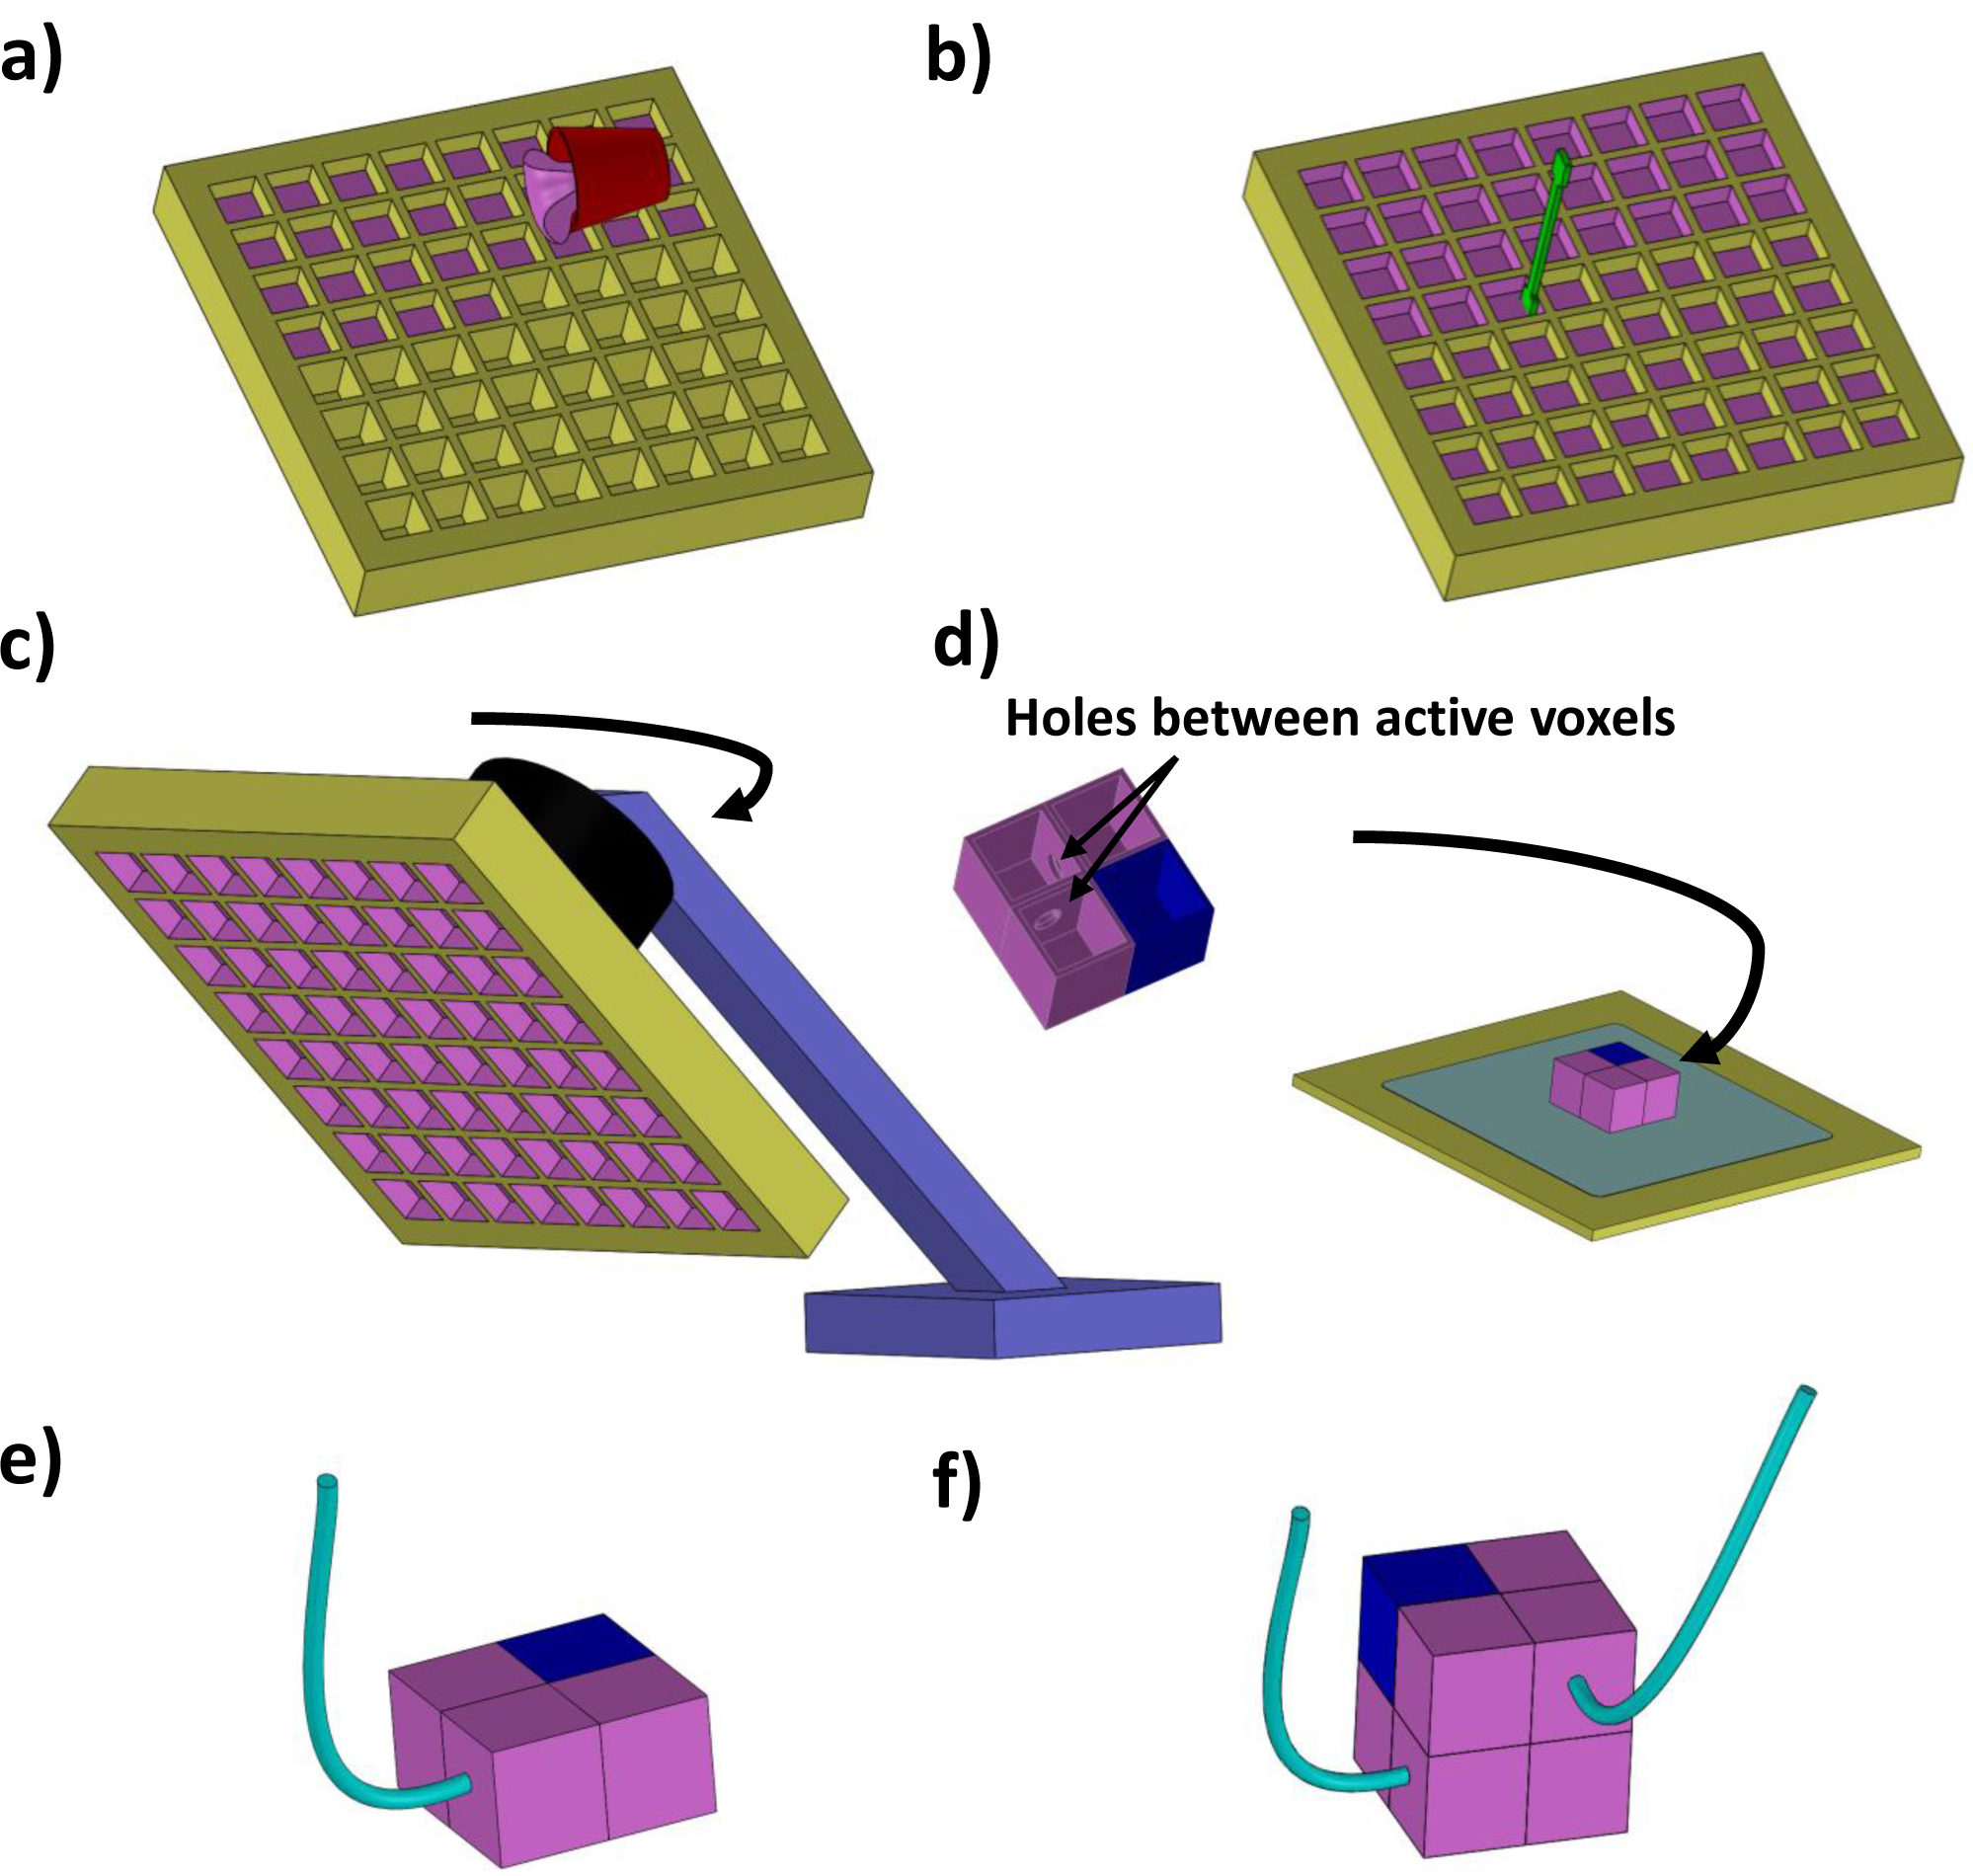
\includegraphics[width=0.7\linewidth]{Chapter02/fig/voxel_manufacturing.jpg}
    % \vspace{0pt}
    \caption{\textbf{Manufacturing modular soft robots.}
    Hollow, silicone voxels were created by partially filling an open-face mold with silicone (\textbf{a}), 
    using a spatula to spread it along the interior walls (\textbf{b}), and then securing the mold to a 1-axis rotational molding machine (\textbf{c}). This process allowed excess silicone to drip out of the mold, while spreading the remaining silicone into a thin uniform layer.
    The cured, bottomless voxels were then appropriately arranged and connected for each x,y slice of the design, and bonded with a shared bottom layer (\textbf{d}).
    Finally, tubing was attached (\textbf{e}), and the slices were stacked and bonded to form the design (\textbf{f}). 
    Video:
\href{https://youtu.be/jbQ2T7jIYRU}{\color{blue}\tt\textbf{youtu.be/jbQ2T7jIYRU}}.
    }
    \label{fig:real}
    % \vspace{-1.5em}
\end{figure}
